
\documentclass{article}
\usepackage{polski}
% \usepackage{babel}
\usepackage{amsmath} % for maths
\usepackage{graphicx} % images
\usepackage{subcaption} % subimages
\usepackage{geometry}
\usepackage{multirow}
\geometry{
	a4paper,
	total={150mm,267mm},
	left=30mm,
	top=15mm,
}
\setcounter{section}{4}

\title{Sprawozdanie nr 2\\Analiza Obrazów}
\date{2019-12-16}
\author{Tomasz Rajchel}
	
	
\begin{document}
	\maketitle
	\pagenumbering{gobble}

	\tableofcontents
	\newpage
	\pagenumbering{arabic}
	
	\section{Laboratorium 5 - Morfologie}
	\subsection{Wstęp}
	\begin{center}
		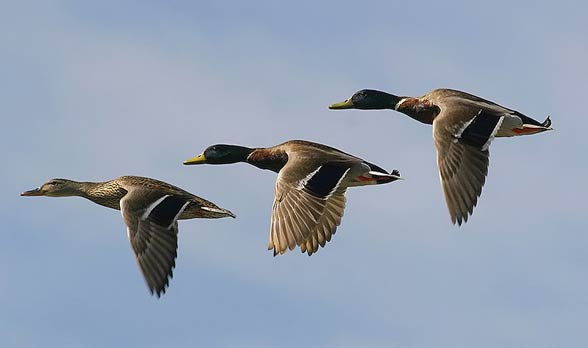
\includegraphics[width=\linewidth]{../../pictures/kaczki.jpg}
		\captionof{figure}{Obraz bazowy}
	\end{center}

	Na obrazie znajdują się 3 obiekty. Musimy jednak oddzielić je od tła. Wykorzystamy do tego binaryzację (z progiem .55 jasności dla obrazu w odcieniach szarości) i operację zamknięcia by pozbyć się "dziur" powstałych w obiektach.
	\begin{center}
		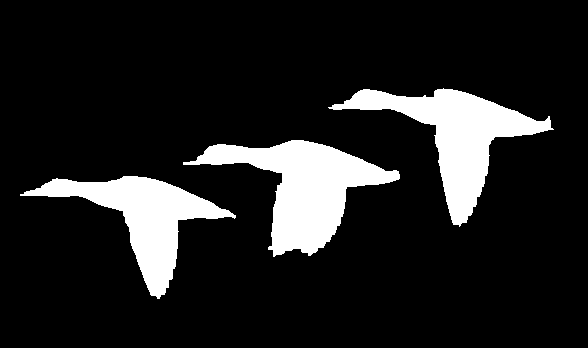
\includegraphics[width=\linewidth]{../../lab05/kaczki_binary_closed.png}
		\captionof{figure}{Oddzielanie obiektów od tła.}
	\end{center}

	\textbf{Liczba Eulera} jest miarą topologii obrazu. Jest definiowana jako całkowita liczba obiektów na obrazie (binarnym) minus liczba dziur w obiektach.
	Manipulując obrazem zależy nam na tym by liczba ta była stała. Nie chcemy zmienić liczby obiektów a jedynie ich kształt. Dla powyższego obrazu liczba Eulera jest równa 3.

	Do wykonywania morfologicznych operacji na obrazach binarnych skorzystamy z funkcji dostępnej w MATLAB'ie o nazwie 'bwmorph'.	
	\subsection{Skel}
	Szkieletowanie usuwa piksele na krawędziach jednocześnie niedopuszczając by obiekt się rozpadł.
	\begin{center}
		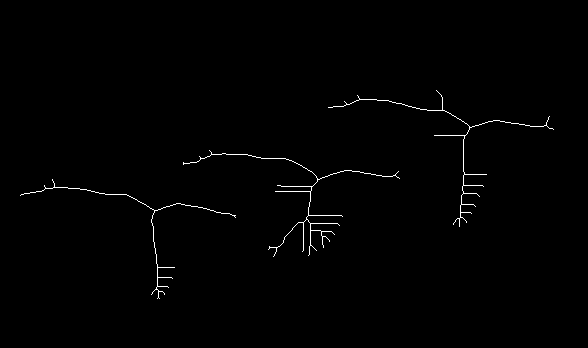
\includegraphics[width=\linewidth]{../../lab05/kaczki_skeleton.png}
		\captionof{figure}{Szkielety obiektów.}
	\end{center}
	
	\subsection{Remove}
	'Remove' usuwa środek obiektów. Zwraca tylko obwód.
	\begin{center}
		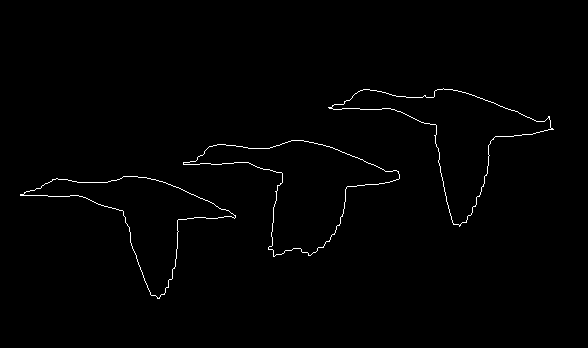
\includegraphics[width=\linewidth]{../../lab05/kaczki_perimeter.png}
		\captionof{figure}{Obwody obiektów.}
	\end{center}

	\subsection{Shrink}
	Operacja 'shrink' zmniejsza obiekt poprzez usuwanie pikseli zaczynając od krawędzi. Warto zaznaczyć, że efekt końcowy nie jest środkiem geometrycznym.
	\begin{center}
		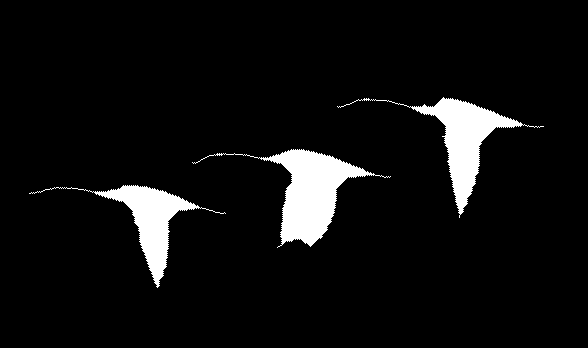
\includegraphics[width=\linewidth]{../../lab05/kaczki_shrink_5.png}
		\captionof{figure}{5 iteracji zmniejszania.}
	\end{center}
	\begin{center}
		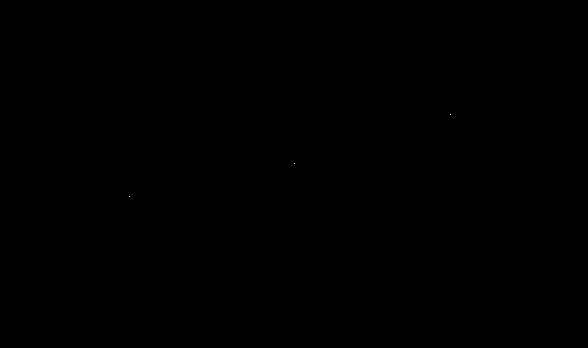
\includegraphics[width=\linewidth]{../../lab05/kaczki_shrink_Inf.png}
		\captionof{figure}{Maksymalna ilość iteracji zmniejszania.}
	\end{center}
	
	\subsection{Thin}
	Operacja pocieniania redukuje obiekty aż do samych linii.
	Ciekawym jej zastosowaniem jest znajdywanie dróg, rzek itp. na zdjęciach satelitarnych.
	\begin{center}
		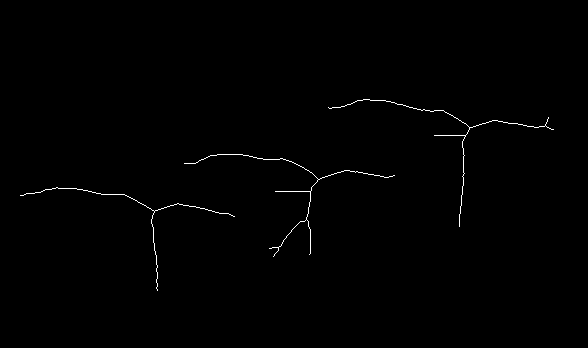
\includegraphics[width=\linewidth]{../../lab05/kaczki_thin.png}
		\captionof{figure}{Wynik operacji pocieniania (maks liczba iteracji)}
	\end{center}
	Możemy użyć funkcji 'branchpoints', która zwróci nam końce linii.
	
	Te punkty mogą okazać się użyteczne do dalszej analizy lub szkolenia sieci neuronowych do rozpoznawania obiektów.
	
	\subsection{Thicken}
	Operacja poszerzania, powiększy nasze obiekty jednak nie pozwoli im się scalić.
	\begin{center}
		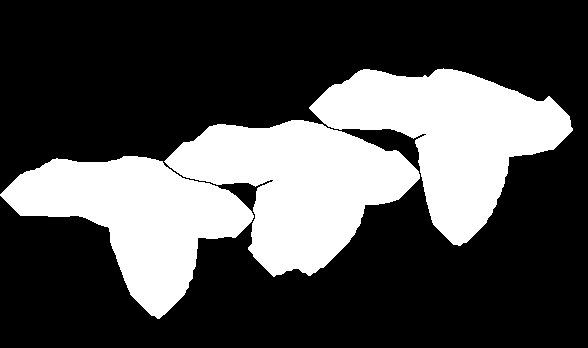
\includegraphics[width=\linewidth]{../../lab05/kaczki_thicken_20.png}
		\captionof{figure}{Wynik operacji poszerzania (20 iteracji)}
	\end{center}
	\begin{center}
		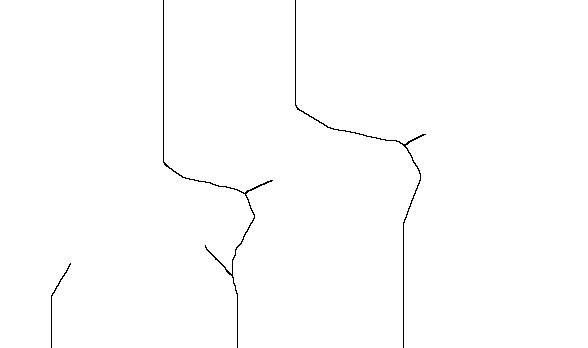
\includegraphics[width=\linewidth]{../../lab05/kaczki_thicken_Inf.png}
		\captionof{figure}{Wynik operacji poszerzania (maks liczba iteracji)}
	\end{center}
	W każdym z tych obszarów na pewno znajduje się jeden obiekt.
	
	\subsection{Oddzielanie obiektów}
	Możemy wykorzystać etykiety do odróżniania obiektów. Dostępna w matlabie funkcja 'bwlabel' zwróci nam macierz ponumerowanych obiektów dla obrazu binarnego.
	\begin{center}
		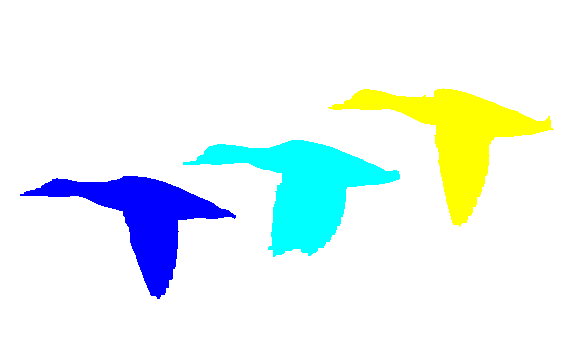
\includegraphics[width=\linewidth]{../../lab05/kaczki_color_label.png}
		\captionof{figure}{Ponumerowane kaczki, oznaczone kolorami.}
	\end{center}

	\subsection{Transformata odległościowa}
	Funkcja 'bwdist' zwraca odległość od najbliższego obiektu dla każdego piksela.
	\begin{center}
		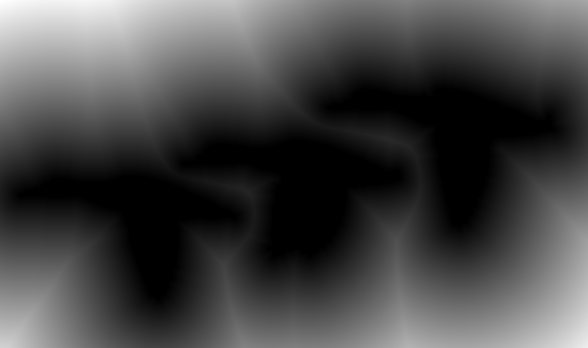
\includegraphics[width=\linewidth]{../../lab05/kaczki_distance.png}
		\captionof{figure}{Wynik operacji 'bwdist'.}
		\label{fig:kaczki_dist}
	\end{center}
	
	\subsection{Segmentacje}
	Korzystając z poprzedniego obrazu (Rysunek \ref{fig:kaczki_dist}). Wykonamy operację segmentacji wododziałowej.
	\begin{center}
		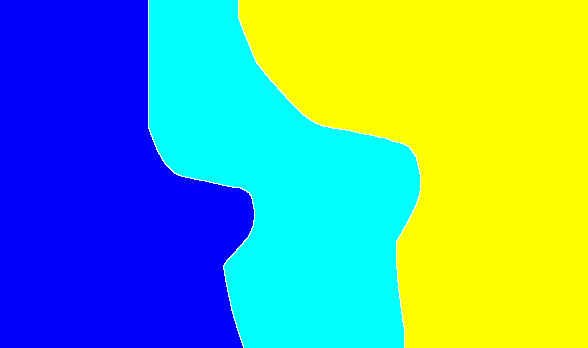
\includegraphics[width=\linewidth]{../../lab05/kaczki_watershed.png}
		\captionof{figure}{Segmentacja wododziałowa.}
	\end{center}	
	W powyższym przykładzie skorzystaliśmy z metryki euklidesowej (najpopularniejsza, zwykła odległość). Ale do niektórych zastosowań lepiej jest skorzystać z innych metryk.
	
	\begin{center}
		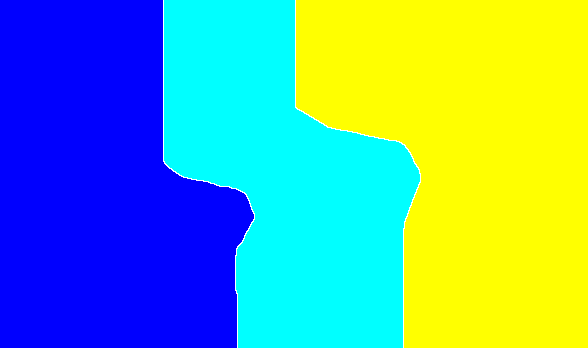
\includegraphics[width=\linewidth]{../../lab05/kaczki_manhattan.png}
		\captionof{figure}{Segmentacja z metryką manhattan.}
	\end{center}

	\begin{center}
		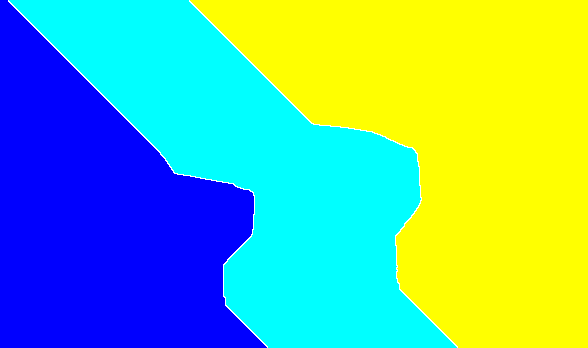
\includegraphics[width=\linewidth]{../../lab05/kaczki_chessboard.png}
		\captionof{figure}{Segmentacja z metryką chessboard.}
	\end{center}
	
	\section{Laboratorium 6 - Współczynniki geometryczne} 
	\subsection{Wstęp}
	\begin{center}
		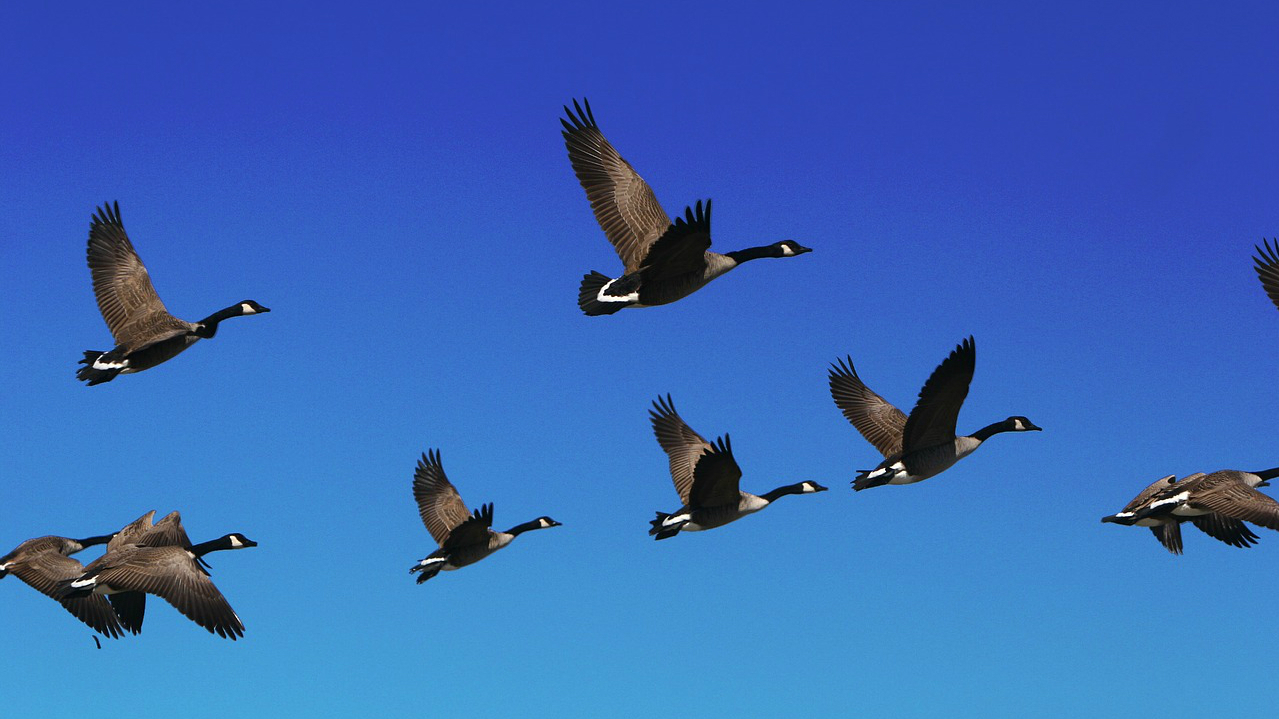
\includegraphics[width=\linewidth]{../../pictures/ptaki.jpg}
		\captionof{figure}{Obraz bazowy - ptaki.jpg}
		\label{fig:ptaki}
	\end{center}

	Można zauważyć, że na powyższym kolorowym (RGB) obrazie największa różnica między obiektami (ptakami) a tłem występuje w kanale niebieskim.
	\begin{center}
		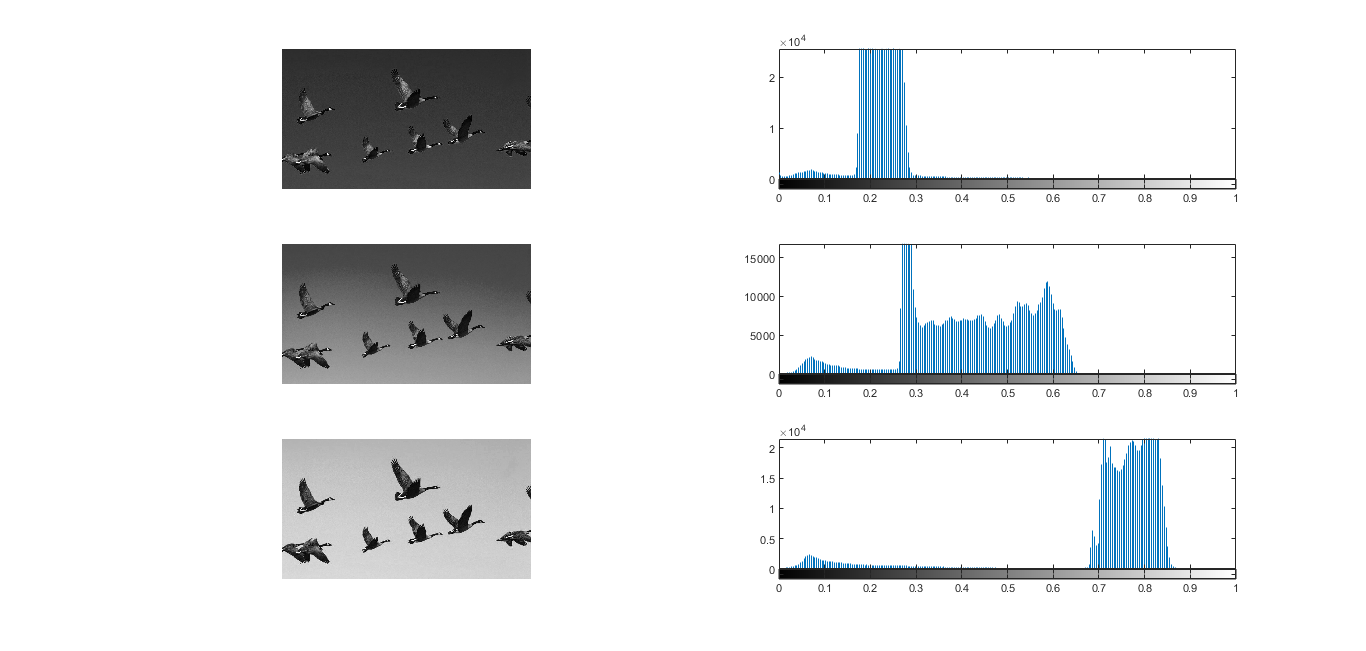
\includegraphics[width=\linewidth]{../../lab06/ptaki_rgb.png}
		\captionof{figure}{Kanały RGB i ich histogramy.}
	\end{center}
	Skorzystamy z tej własności, żeby lepiej odseparować obiekty od tła.
	
	\begin{center}
		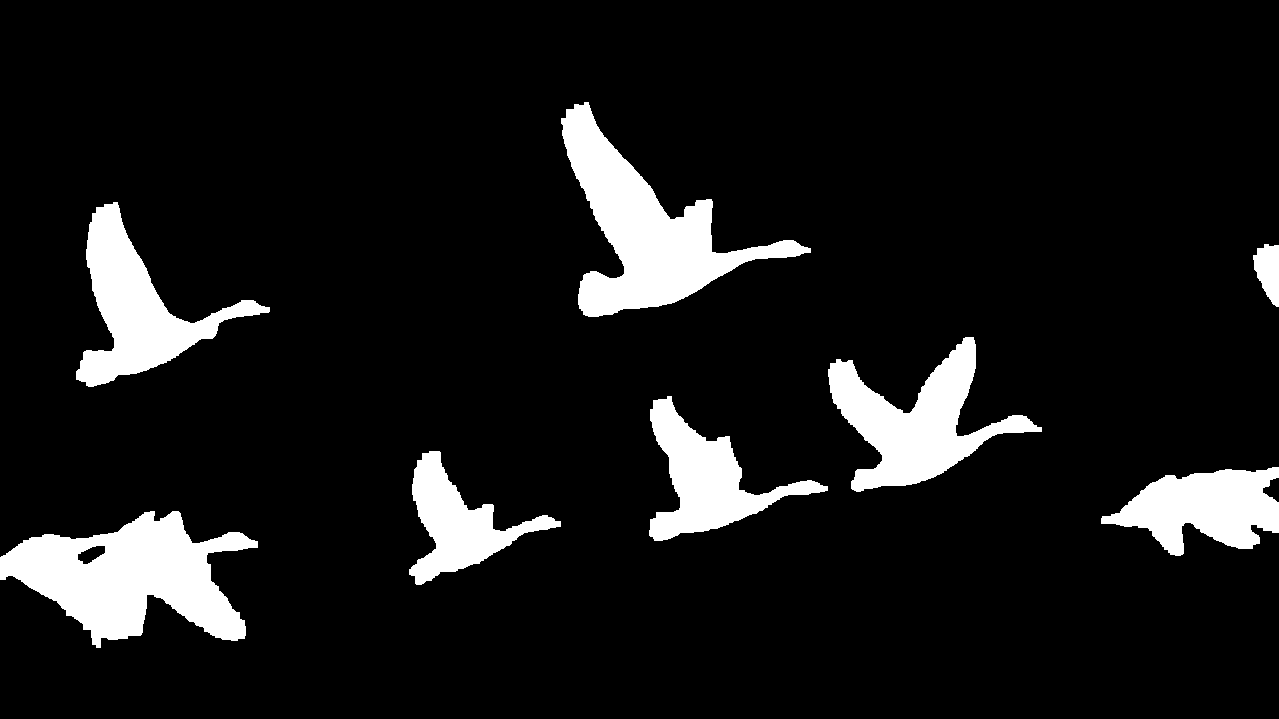
\includegraphics[width=\linewidth]{../../lab06/ptaki_bim.png}
		\captionof{figure}{Obraz binarny, progowanie w kanale niebieskim.}
	\end{center}

	\subsection{Współczynniki dostępne w MATLAB'ie}
	Udało nam się wykryć 8 obiektów, w tym dwa scalone i jeden urywek. Możemy dla nich obliczyć różne współczynniki. Funkcja 'regionprops' w matlabie zwraca 23 parametry. Niektóre z nich to:
	\begin{enumerate}
		\item Area - Pole powierzchni
		\item Centroid - Środek geometryczny
		\item BoundingBox - najmniejszy ograniczający kwadrat z bokami równoległymi do osi X i Y.
		\item MajorAxisLength - Długość osi wielkiej
		\item MinorAxisLength - Długość osi małej
		\item Eccentricity - Mimośród
		\item Orientation - Skierowanie
		\item EulerNumber - Liczba Eulera
		\item Perimeter - Obwód
	\end{enumerate}
	Im więcej współczynników tym więcej 'wymiarów' w których obiekty się od siebie różnią. Główną ideą obliczania tych współczynników jest łatwiejsze odróżnianie od siebie obiektów.
	
	Dla wielu współczynników punktem odniesienia jest koło (np. mimośród).

	\subsection{Dodatkowe współczynniki}
	Zdefiniujemy funkcje obliczające następujące współczynniki:
	\begin{enumerate}
		\label{coefficients}
		\item Kształt
		\item Współczynnik Malinowskiej
		\item Współczynnik Haralick'a
		\item Średnica Feret'a
			- stosunek średnic z bounding box (bok poziomy do boku pionowego)
		\item Współczynnik Danielsson'a
			- Średnia odległość piksela od krawędzi, dla koła największa możliwa wartosć
		\item CircularityS (Kolistość)
		\item CircularityL (Kolistość)
		\item Współczynnik Blair'a - Bliss'a
			- średnia odległość od środka dla każdego piksela
		
	\end{enumerate}

	Wykorzystamy obliczone współczynniki by pozbyć się obiektów odstających od średniej (scalone ptaki i urywki).
	
	\begin{table}
		\begin{center}
			\begin{tabular}{c|c|c|c|c|c|c|c}
				\multicolumn{8}{c}{Współczynniki}\\
				1 & 2 & 3 & 4 & 5 & 6 & 7 & 8\\
				\hline
				3.29 & 0.81 & 81.22 & 0.53 & 103.88 & 154.72 & 280.75 & 6.98 \\
				2.93 & 0.71 & 73.24 & 0.95 & 92.18  & 123.21 & 211.04 & 6.00 \\
				2.99 & 0.73 & 55.15 & 0.88 & 87.10  & 96.88  & 167.43 & 5.45 \\
				3.21 & 0.79 & 88.29 & 0.86 & 103.31 & 150.73 & 269.93 & 6.65 \\
				3.15 & 0.78 & 63.63 & 0.81 & 84.69  & 108.62 & 192.90 & 5.77 \\
				3.60 & 0.90 & 70.93 & 0.72 & 114.52 & 127.92 & 242.55 & 6.25 \\
				2.45 & 0.57 & 59.25 & 0.50 & 73.63  & 109.92 & 172.21 & 5.93 \\
				1.62 & 0.27 & 20.73 & 2.48 & 17.62  & 38.01  & 48.38  & 3.45 \\
			\end{tabular}
		\end{center}
	\end{table}

	\begin{center}
		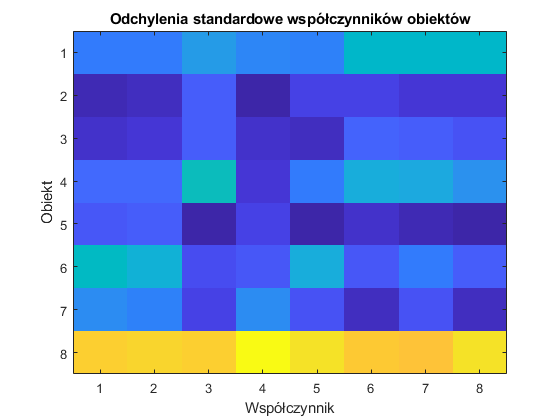
\includegraphics[width=\linewidth]{../../lab06/ptaki_err.png}
		\captionof{figure}{Odchylenie standardowe dla różnych obiektów}
	\end{center}
	Jak widać udało nam się zdecydowanie wykluczyć tylko obiekt nr 8 (skrawek, widoczny po prawej stronie). 
	
	Potrzebna nam jest metoda która może nauczyć się odróżniać od siebie różne obiekty korzystając z obliczonych parametrów.
	
	\section{Laboratorium 7 - Klasyfikacja obiektów przy użyciu sieci neuronowych}
	\subsection{Wstęp}
	\begin{center}
		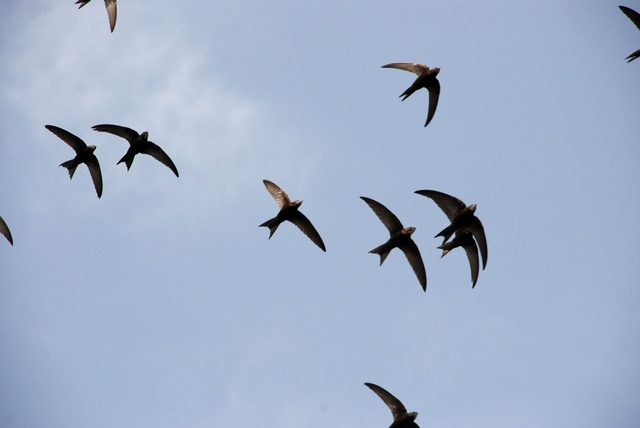
\includegraphics[width=\linewidth]{../../pictures/ptaki2.jpg}
		\captionof{figure}{Obraz bazowy - ptaki2.jpg}
		\label{fig:ptaki2}
	\end{center}
	Korzystając ze współczynników przedstawionych w poprzednim rozdziale, nauczymy sieć neuronową odróżniać ptaki z z obrazu \ref{fig:ptaki} od ptaków z obrazu \ref{fig:ptaki2}.
	
	\begin{center}
		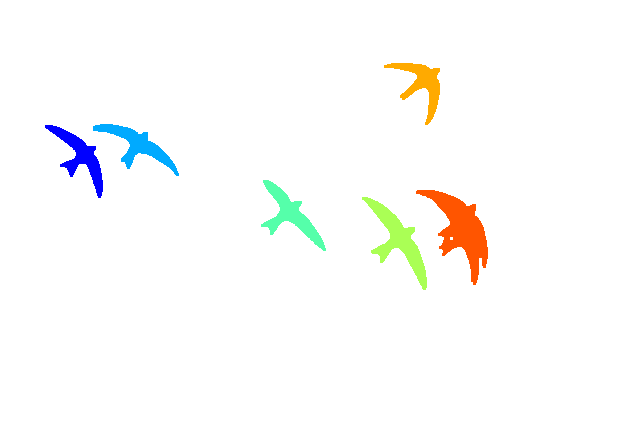
\includegraphics[width=\linewidth]{../../lab07/ptaki2_label.png}
		\captionof{figure}{Wykryte, pełne obiekty - ptaki2.}
	\end{center}

	\subsection{Uczenie sieci neuronowej}
	Wejściem sieci bedą współczynniki z podpunktu \ref{coefficients}.
	
	Zero na wyjściu sieci oznacza obiekt z obrazu 'ptaki.jpg', natomiast jedynka obiekt z obrazu 'ptaki2.jpg'.
	
	\begin{center}
		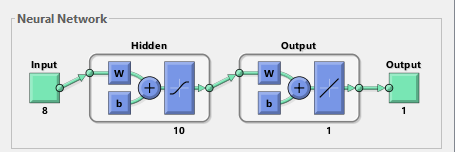
\includegraphics[width=\linewidth]{../../lab07/neural_net.png}
		\captionof{figure}{Struktura sieci neuronowej.}
	\end{center}

	\begin{center}
		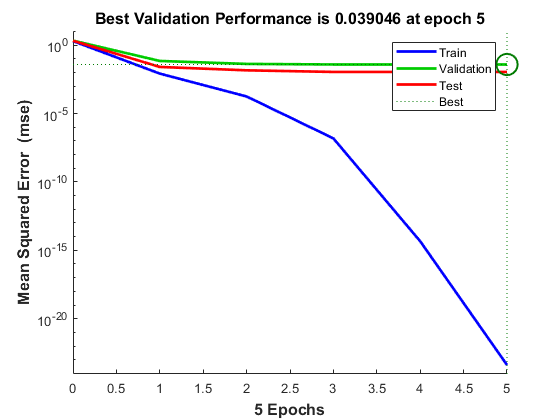
\includegraphics[width=\linewidth]{../../lab07/nn_performance.png}
		\captionof{figure}{Historia wydajności sieci podczas szkolenia.}
	\end{center}
	Widzimy, że na takim miniaturowym zbiorze danych uczenie kończy się już w piątej epoce. Dalej następuje jedynie poprawa na zbiorze uczącym 'Train' - tak zwane przeuczenie.
	
	Sprawdźmy jak dobrze nasza sieć klasyfikuje obiekty. Na wejście podamy 8 elementową macierz współczynników obliczonych dla obiektów z obrazu 'ptaki.jpg' i 6 elementową macierz współczynników dla obiektów z obrazu 'ptaki2.jpg'. Połączone w macierzy 'ucz'.
	\begin{center}
		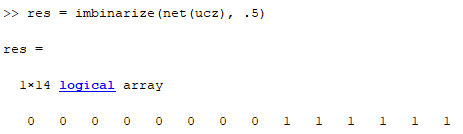
\includegraphics[width=\linewidth]{../../lab07/output.png}
		\captionof{figure}{Wyjście z sieci neuronowej dla obiektów ptaki i ptaki2.}
	\end{center}
	Widzimy, że nasza sieć prawidłowo sklasyfikowała wszystkie obiekty.
	
\end{document}